\documentclass[a4paper,11pt]{article}
\usepackage[utf8]{inputenc}
\usepackage{subfigure}
\usepackage{rotating}
\usepackage{nicefrac}
\usepackage{float}
\usepackage{amsmath}
\usepackage{amssymb}
\usepackage{hyperref}
\usepackage[export]{adjustbox}
\usepackage[T1]{fontenc}
\usepackage{enumitem}
\usepackage{lstautogobble}		% Pour mettre à gauche le code
\usepackage{listings}			% Pour afficher du code
\usepackage{graphicx} 			% Pour l'affichage d'images
\usepackage{titling} 			% Reduit l'espace au dessus du titre et auteurs
\usepackage[left=20mm,top=10mm, right=18mm, bottom=10mm, includefoot]{geometry}
\usepackage[hmargin=2cm,vmargin=2cm]{geometry}
\setlength{\droptitle}{-2em}   % Reduit l'espace au dessus du titre et auteurs

\title{\textsc{[INFO-H-303] Bases de données - Rapport Projet:}\
   "Ebay"}
\author{Alexandre Heneffe - 000440761\\
        Nicolas Jonas - 000442112}
\date{Mars 2018}

\begin{document}
\maketitle
\section{Introduction}

Ceci est le rapport du projet de base de données. Celui-ci contiendra le schéma entité-relationnel (et ses contraintes) de la future base de données ainsi que sa traduction en un modèle relationnel.

\subsection{Hypothèses}

\begin{itemize}[label=\textbullet]
	\item Un objet appartient au minimum à 1 catégorie
	\item Une catégorie peut exister sans objet y étant associée
	\item Chaque objet est unique, il n'y a pas de notion de quantité
	\item Un utilisateur doit être majeur afin d'acheter des objets

\end{itemize}

\subsection{Contraintes d'intégrités}

\begin{itemize} [label=\textbullet]
	\item La date de vente d'un objet doit être > à la date de mise en vente de cet objet
	\item Le prix proposé pour une proposition d'achat doit être >= au prix minimum de l'objet
	\item Un administrateur ne peut pas se supprimer lui-même
	\item L'évaluation d'un objet est faite que si cet objet est acheté depuis moins de 10 jours, c'est-à-dire que la date d'évaluation doit être < à
	la date de vente de l'objet + 10
	\item La date d'évaluation d'un objet doit être > à la date de vente d'un objet
	\item Le pseudo d'un utilisateur est unique (c'est ce qui permet de différencier les utilisateurs)
	\item Le vendeur d'un objet ne peut pas être l'acheteur de cet objet
	\item la date de naissance d'un vendeur doit être > à la date de mise en vente d'un objet qu'il vend
	\item la note d'une évaluation est une valeur entre 1 et 10
	\item le numéro d'une évaluation doit être unique
	
\end{itemize}

\section{Modèle Entité-Association}
\subsection{Schéma}
\begin{center}
  \begin{sidewaysfigure}
    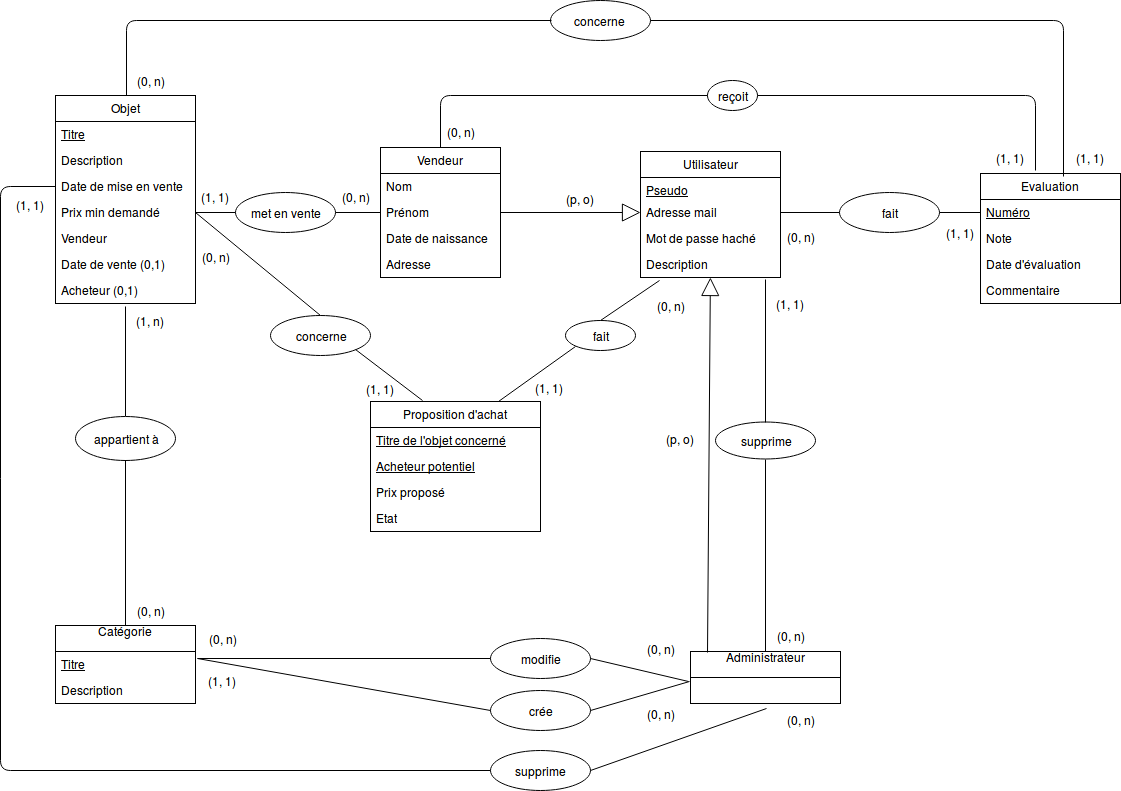
\includegraphics[width = 25cm]{schemaEA}
  \end{sidewaysfigure}
\end{center}

\newpage

\subsection{Justifications}
La généralisation (Utilisateur, vendeur et administrateur) dans le schéma, est partiel et couvrant.
\begin{itemize}
\item Partiel: Les vendeurs et administrateurs sont des types d'utilisateurs. Mais il y a aussi les utilisateurs classiques.
\item Couvrant: Un utilisateur peut être à la fois vendeur et administrateur par exemple.
\end{itemize}

\textbf{Evaluations :} une évaluation a pour clef un Numéro (qui doit donc être unique) car ses autres attributs ne permettent pas de la
	      distinguer de manière unique (ex : deux évaluations peuvent avoir la même note et la même date).

\textbf{Utilisateur :} un utilisateur quelque soit son statut (simple utilisateur, vendeur et/ou administrateur) reste toujours identifié
par son Pseudo.

\textbf{Proposition d'achat :} un proposition d'achat est identifiée à la fois par le Titre de l'objet concerné et par l'Acheteur potentiel,
car on ne peut se baser uniquement sur le Titre de l'objet (il peut y avoir plusieurs propositions d'achat pour un même objet)
ou sur le Pseudo de l'acheteur potentiel (un acheteur peut faire plusieurs propositions d'achats sur différenets Objets).

\section{Modèle Relationnel}
Dans cette section, nous traduisons le modèle entité-association de la section précédente en un modèle relationnel et en ajoutant ses contraintes.

\subsection{Modèle}

\indent

\paragraph{Objet} (\underline{Titre}, Description, DateMiseEnVente, PrixMin, Vendeur, DateVente, Acheteur, NumVendeur, NumAdmin)\\
\indent - Objet.NumVendeur référence Vendeur.Numéro\\
\indent - Objet.NumAdmin référence Administrateur.Numéro


\paragraph{Vendeur} (\underline{Pseudo}, Nom, Prénom, DateNaissance, Adresse, PseudoUser)\\
\indent - Vendeur.PseudoUser référence Utilisateur.Pseudo

\paragraph{Administrateur} (\underline{Pseudo}, PseudoUser)\\
\indent - Administrateur.PseudoUser référence Utilisateur.Pseudo


\paragraph{Utilisateur} (\underline{Pseudo}, AddresseMail, MotDePasse, 
Description, PseudoAdmin)\\
\indent - Utilisateur.PseudoAdmin référence Administrateur.Pseudo


\paragraph{PropositionAchat} (\underline{NuméroObjet}, \underline{Acheteur}, Prix, Etat, TitreObj, PseudoUser)\\
\indent - PropositionAchat.TitreObj référence Objet.Titre\\
\indent - PropositionAchat.PseudoUser référence Utilisateur.Pseudo


\paragraph{Evaluation} (\underline{Numéro}, Note, Date, Commentaire, TitreObj, PseudoVendeur, PseudoUser)\\
\indent - Evaluation.TitreObj référence Objet.Titre\\
\indent - Evaluation.PseudoVendeur référence Vendeur.Pseudo\\
\indent - Evaluation.PseudoUser référence Utilisateur.Pseudo


\paragraph{Catégorie} (\underline{Titre}, Description, PseudoAdmin)\\
\indent - Catégorie.PseudoAdmin référence Administrateur.Pseudo


\paragraph{Appartenance} (\underline{TitreObj, TitreCatégorie})\\
\indent - Appartenance.TitreObj référence Objet.Titre\\
\indent - Appartenance.TitreCatégorie référence Catégorie.Titre


\paragraph{Modifiation} (\underline{TitreCatégorie, PseudoAdmin})\\
\indent - Modification.TitreCatégorie référence Catégorie.Titre\\
\indent - Modification.PseudoAdmin référence Administrateur.Pseudo


\subsection{Contraintes}

\begin{itemize}
\item Pour tout Objet.Titre, il existe au moins un Appartenance.TitreObj
\item Pour un Objet, Objet.DateVente > Objet.DateMiseEnVente
\item Pour un PropositionAchat, PropositionAchat.Prix >= Objet.PrixMin
\item Pour un Utilisateur, Administrateur.Pseudo != Utilisateur.Pseudo (un Administrateur ne peut pas se supprimer)
\item Pour un Evaluation, Evaluation.Date < Objet.DateVente + 10
\item Pour un Evaluation, Evaluation.Date > Objet.DateVente
\item Pour un Vendeur, Vendeur.DateNaissance >= 18
\item Pour un Vendeur, Vendeur.DateNaissance > Objet.DateMiseEnVente
\item Pour un Objet, Objet.Vendeur != Objet.Acheteur
\end{itemize}


\end{document}